% Build: make beamer   (XeLaTeX or LuaLaTeX; see ../../README.md)
\documentclass[aspectratio=169,11pt]{beamer}
\usetheme{kentigern}          % \usetheme[light]{kentigern} for the Parchment version
\usepackage{booktabs}

\title{GWTC-5.0 \& Beyond}
\subtitle{Updated transients observations and results from O4}
\author{Daniel Williams}
\institute{Institute for Gravitational Research, University of Glasgow\\
For the LIGO-Virgo-KAGRA Collaboration}

\begin{document}

\begin{frame}[plain]
  \titlepage
\end{frame}

\begin{frame}{What is GWTC-5.0?}
  \begin{itemize}
    \item The fifth version of the Gravitational-Wave Transient catalogue
    \begin{itemize}\item The GWTC is a cumulative catalogue\end{itemize}
    \item Provides parameter information for all candidates in O1 -- O4b
    \item This update contains new candidates from O4b
  \end{itemize}
\end{frame}

\kentigernstat{291}{New candidates (O4a+O4b)}

\begin{frame}{Source masses}
  \kentigernref{arxiv.org/abs/2605.27225}
  \begin{columns}[T]
    \begin{column}{0.4\textwidth}
      \begin{itemize}
        \item GW231123 (O4a) remains the heaviest event we've yet observed.
        \item \textbf{Four O4b events} may have produced intermediate-mass BH remnants.
      \end{itemize}
    \end{column}
    \begin{column}{0.56\textwidth}
      \kentigernpanel{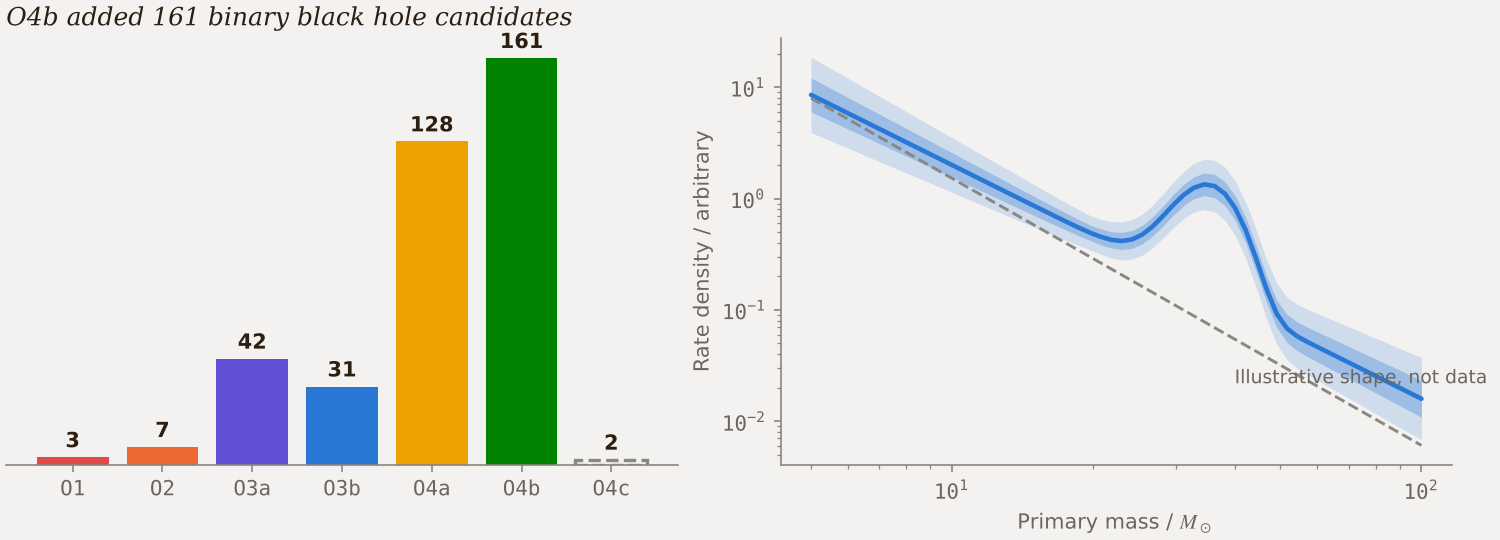
\includegraphics[width=\linewidth]{example-figure.png}}
    \end{column}
  \end{columns}
\end{frame}

\begin{frame}{O1 -- O4 scorecard}
  \small
  \begin{tabular}{@{}llrrr@{}}
    \toprule
    Observing run & Catalogue update & BBH & NSBH & BNS\\
    \midrule
    O1 & GWTC-1.0 & 3 & 0 & 0\\
    O2 & GWTC-1.0 & 7 & 0 & 1\\
    O3a & GWTC-2.1 & 42 & 2 & 1\\
    O3b & GWTC-3.0 & 31 & 4 & 0\\
    O4a & GWTC-4.0 & 128 & 2 & 0\\
    \alert{O4b} & \alert{GWTC-5.0} & \alert{161} & \alert{0} & \alert{0}\\
    O4c & GWTC-6.0 & 2* & -- & --\\
    \bottomrule
  \end{tabular}
\end{frame}

\kentigernthanks[qr-site.png]{daniel-williams.co.uk}

\end{document}
